\documentclass[11pt,a4paper]{article}
\usepackage{fontspec}
\setmainfont{TeX Gyre Pagella}
\newfontfamily\headfont{Inter}[UprightFont=*-ExtraBold,BoldFont=*-ExtraBold,Extension=.otf,Path=/usr/share/fonts/opentype/inter/]
\usepackage[a4paper,margin=2.3cm]{geometry}
\usepackage{graphicx,booktabs,float,caption,array,xcolor,longtable}
\usepackage{xurl}
\usepackage[hidelinks]{hyperref}
\usepackage{titlesec}
\usepackage[round]{natbib}
\usepackage{setspace}
\setstretch{1.05}
\renewcommand{\topfraction}{0.9}
\renewcommand{\bottomfraction}{0.8}
\renewcommand{\textfraction}{0.1}
\renewcommand{\floatpagefraction}{0.75}
\setlength{\parindent}{0pt}
\setlength{\parskip}{0.55em}
\titleformat{\section}{\headfont\Large}{\thesection}{0.8em}{}
\titleformat{\subsection}{\headfont\large}{\thesubsection}{0.8em}{}
\captionsetup{font=small,labelfont=bf}
\urlstyle{same}
\hypersetup{pdftitle={Not Where It Says on the Ticket},pdfauthor={Tristan Hotham}}

\begin{document}
\begin{center}
{\Large\bfseries Not Where It Says on the Ticket\par}
\vspace{0.4em}
{\large Airports and railway stations far from the places they are named after, from Wikidata and OpenStreetMap\par}
\vspace{1.2em}
{\large Tristan Hotham\par}
\vspace{0.3em}
{\small Independent researcher\\
ORCID: 0000-0003-4931-9349\\
DOI: https://doi.org/10.5281/zenodo.24087597\par}
\vspace{0.8em}
2026
\end{center}

\begin{quote}
\small
\begin{center}\textbf{Abstract}\end{center}
Airports and railway stations carry the names of places, and sometimes the place is a long way off. I measure the straight-line distance from 4,448 airports with an IATA code to the places they are named after, using Wikidata's places served, airport labels, Natural Earth towns and 11 names under which airlines sell secondary airports, and from 2,888 railway stations and halts in the United Kingdom to the settlement that begins their name. Half the airports lie within 5.6 km of their namesake and 3.3\% lie more than 30 km away. The farthest confirmed cases are Châlons Vatry, sold as Paris-Vatry (136.1 km from Paris), Chicago Rockford (126.3 km), Tongren Dejiang (110.0 km), Frankfurt-Hahn (103.2 km) and Memmingen, sold as Munich West (100.6 km); twelve of the fifteen farthest are second airports for a city that has a closer one. In Britain, London Oxford Airport is 90.0 km from London. Stations are tighter: half lie within 0.58 km of the settlement in their name and 169 lie 2 km or more away, the farthest being airport stations, parkways and the Victorian ``Road'' stations, of which 9 are named after a village 2 km or more distant. Because rankings concentrate data errors, every airport case of 40 km or more and every station match of 3 km or more was read by eye: 41.6\% of the 113 airport cases and 79.0\% of the 286 station matches were wrong links, homonyms, streets, regions or unresolved.

\textbf{Keywords:} airports; railway stations; place names; secondary airports; low-cost airlines; Wikidata; OpenStreetMap; data quality
\end{quote}

\section{Introduction}
A ticket to Frankfurt that lands at Hahn, in the Hunsrück hills, is a familiar complaint about low-cost air travel. Many airports named after a city some way off took those names in the 1990s and 2000s, when low-cost airlines moved into former military fields and regional airports and sold them under the name of the nearest large city. Railway names stretch too: the Victorian companies built stations named ``Road'' for villages some distance down the road, and the modern railway has its parkways and airport stations. This paper asks how far the names stretch. It measures, for every airport in Wikidata with an IATA code and for every railway station in the United Kingdom in OpenStreetMap, the distance to the place in its name, and ranks the far cases.

A ranking is only as good as its head, and the head of a ranking by distance is where data errors collect: a link to the wrong town of the same name, a coordinate in the wrong hemisphere, a district standing in for a city. The method therefore pairs simple automatic matching with a complete reading by eye of every long case, and the overrides are released with the data.

\section{Data}
\textbf{Airports.} A Wikidata query (run with QLever; \citealt{bast2017}) returned 11,042 airports with an IATA or ICAO code and coordinates, of which 7,963 have an IATA code, with country, annual passengers where recorded (4,602 airports; I take the largest recorded annual value), and each place served (property P931) with its label, coordinates and population. The rows come one per combination of values, so I aggregated them to one record per airport and one per airport and place. Wikidata is a collaboratively edited knowledge base \citep{vrandecic2014}.

\textbf{Stations.} OpenStreetMap \citep{haklay2008} nodes and ways in the UK tagged \texttt{railway=station} or \texttt{railway=halt}, with their name, three-letter CRS code where tagged, and first coordinate: 3,576 stations after merging points of the same name within 1 km, 2,849 of them with a CRS code (National Rail). The rest are heritage, metro, tram and miniature railway stations, and stations in Northern Ireland, where CRS codes are not tagged.

\textbf{Settlements and towns.} Wikidata settlements in the UK with coordinates, population and type (village, hamlet, town, city, suburb and similar), and Natural Earth populated places and countries \citep{naturalearth}.

\section{Methods}
\subsection{Airports and their namesakes}
An airport's namesake must be a place it is named after, not just a place it serves: Wikidata's places served include regions, islands and, for some airports, a list of destinations. A place served counts as a namesake when its English label, or a short form of it (``Freiburg'' for Freiburg im Breisgau), appears as whole words in the airport's English label. Where no place served carries a name in the label, a Natural Earth town of the same country whose name is in the label also counts, if it lies within 150 km (a town of the same name farther away is a namesake by chance); such towns are matched to the Wikidata place of the same name within 30 km where one exists, so that all the airports named after one city are grouped. Because Wikidata labels several secondary airports by their local names, I added 11 names under which airlines have sold them (Table~\ref{tab:mk}). When an airport names several places, it is ranked by the farthest. Distances are great-circle distances from the airport's point to the nearest of the place's points. An airport is a \emph{second airport} for its city when another airport named after the same city is closer to it. For a measure relative to city size, I divide the distance by the radius of a notional circle holding the city's population at 3,000 people per km$^2$ (cities of 100,000 or more).

\subsection{Stations and their namesakes}
Each station name is split into parts at ``and'', ``\&'', ``for'' and ``/''. In each part, the longest run of leading words that is the normalised name of a UK settlement is the candidate namesake; settlements are also indexed under common short forms (Southend for Southend-on-Sea, Builth for Builth Wells, Harling for East Harling, Burton for Burton upon Trent), which are used only if they are more than 5 km nearer than any full-name match. Where a station's whole name is itself a village that grew round it (Builth Road, Clarbeston Road), the village named in it is also looked for. The station is measured to the nearest settlement of that name, and its namesake is the farthest of its parts. I also report the distance beyond a notional circle round the settlement, sized by its population at 3,000 people per km$^2$, so that stations inside big cities do not dominate.

\subsection{Checks by eye}
Every airport namesake of 40 km or more with an IATA code (113 cases) and every station match of 3 km or more (286) was read by eye and given a verdict, recorded in \texttt{code/overrides\_airports.csv} and \texttt{code/overrides\_stations.csv}: kept, a wrong link or coordinate, a region or island, a homonym, a street, or unsure. Only kept cases enter the rankings.

\section{Results}
\subsection{How far airports stand from their names}
Half of the 4,448 airports lie within 5.6 km of the place they are named after; 3.3\% are more than 30 km away, 33 are 50 km or more and 15 are 80 km or more away (Figure~\ref{fig:spread}). The median is shortest in South America and Africa and longest in Asia and Europe (Table~\ref{tab:cont}).

\begin{figure}[tbp]\centering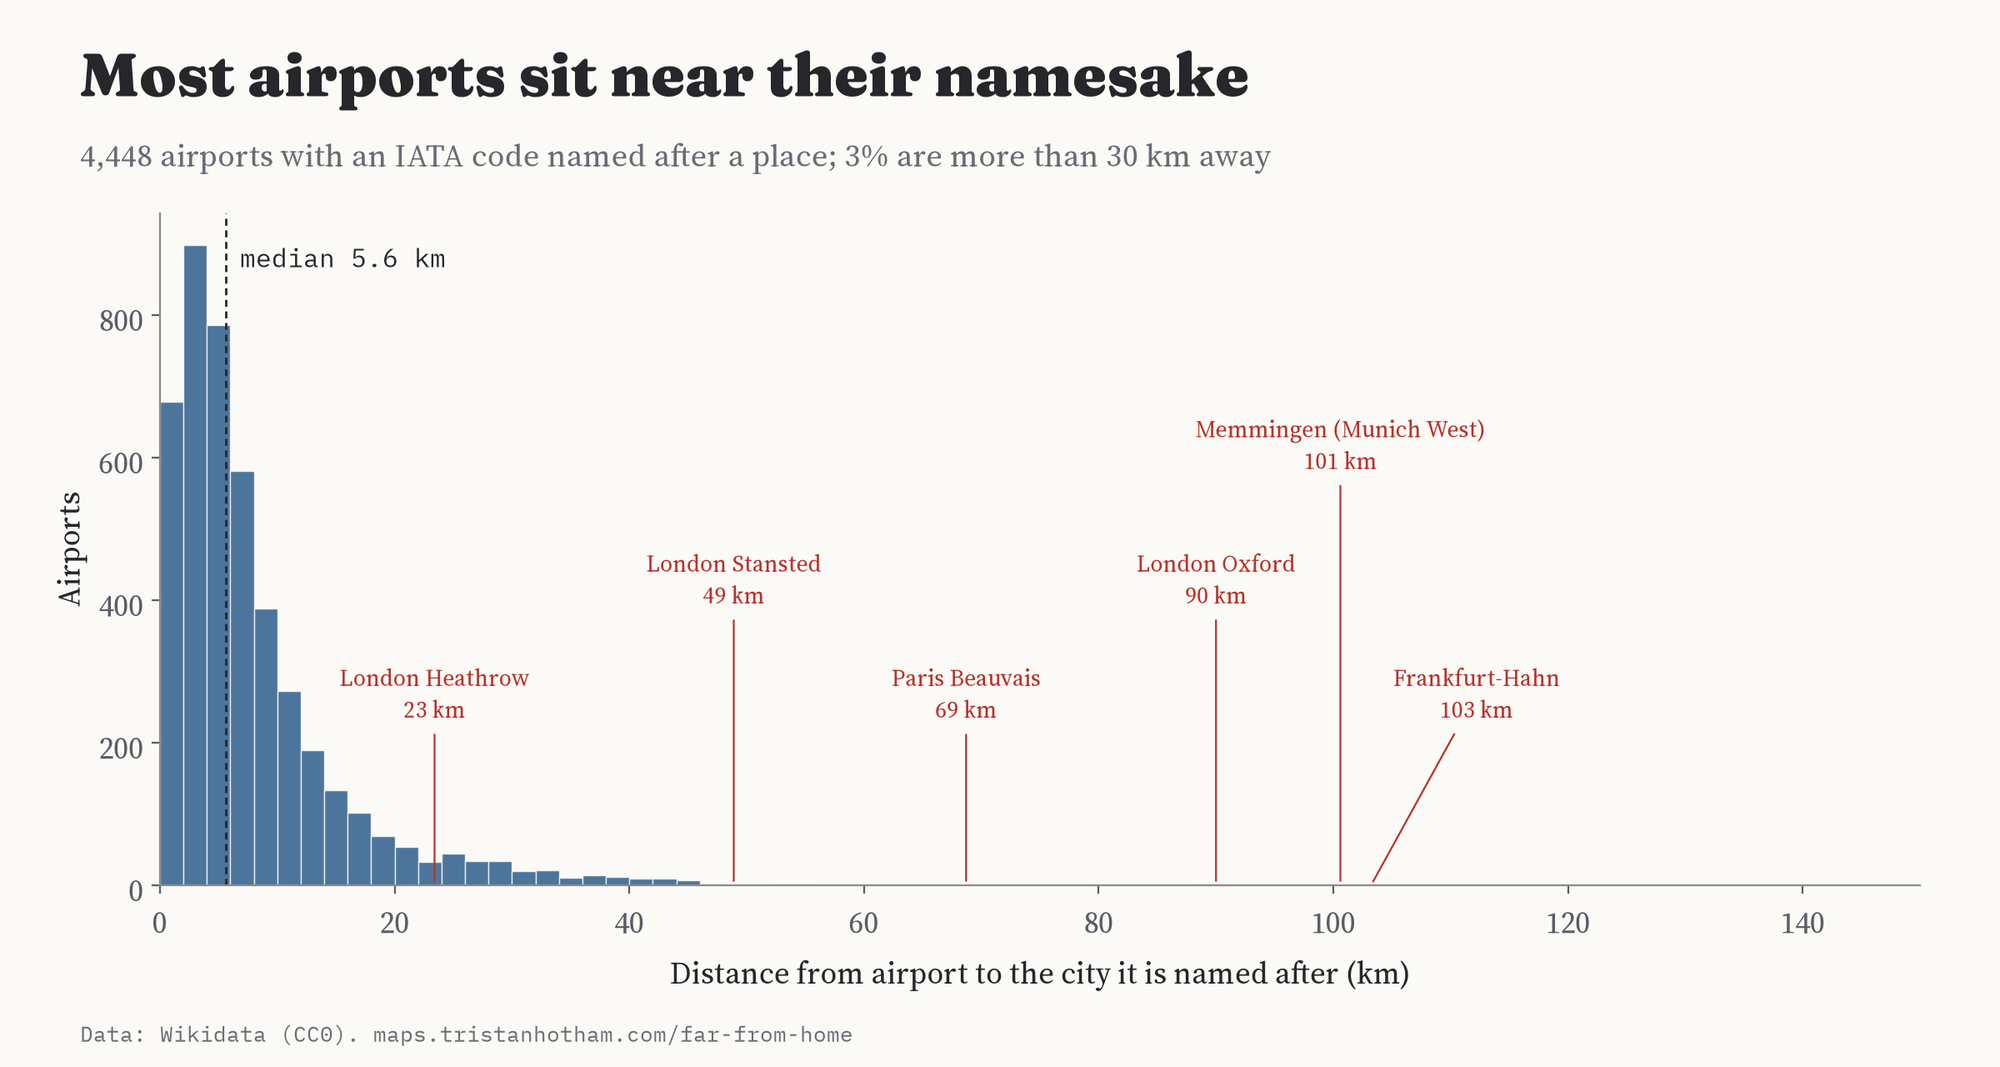
\includegraphics[width=\linewidth]{f_spread.png}\caption{Distance from each airport to the place it is named after.}\label{fig:spread}\end{figure}

\begin{table}[tbp]\centering\small\caption{Median distance from airport to namesake by continent (Natural Earth continents; at least 50 airports).}\label{tab:cont}\begin{tabular}{lrr}\toprule Continent & Airports & Median km\\\midrule
South America & 400 & 3.9\\
Africa & 618 & 4.3\\
North America & 1,470 & 4.9\\
Oceania & 271 & 5.0\\
Europe & 824 & 7.3\\
Asia & 859 & 8.6\\
\bottomrule\end{tabular}\end{table}

The farthest confirmed cases (Figure~\ref{fig:world}, Table~\ref{tab:world}) are Châlons Vatry in Champagne, sold as Paris-Vatry, 136.1 km from Paris; Chicago Rockford, 126.3 km from Chicago; Tongren Dejiang, 110.0 km from Tongren; Frankfurt-Hahn, 103.2 km from Frankfurt; and Memmingen, sold as Memmingen (Munich West), 100.6 km from Munich. Twelve of the fifteen farthest are second airports: Stockholm Skavsta is 11.4 times as far from Stockholm as Bromma, and Hahn 8.8 times as far from Frankfurt as Frankfurt Airport. The three exceptions show other habits: Chinese airports are often named after the prefecture-level city as well as the county they stand in (Shaoyang Wugang, 95.7 km from Shaoyang); New York Stewart, 88.4 km from New York, is the only New York airport with the city in its English label in Wikidata (Kennedy, LaGuardia and Newark are linked to the city but not named after it); and Rize-Artvin, which serves two Turkish provinces from the Black Sea coast, is 81.4 km from Artvin.

\begin{figure}[tbp]\centering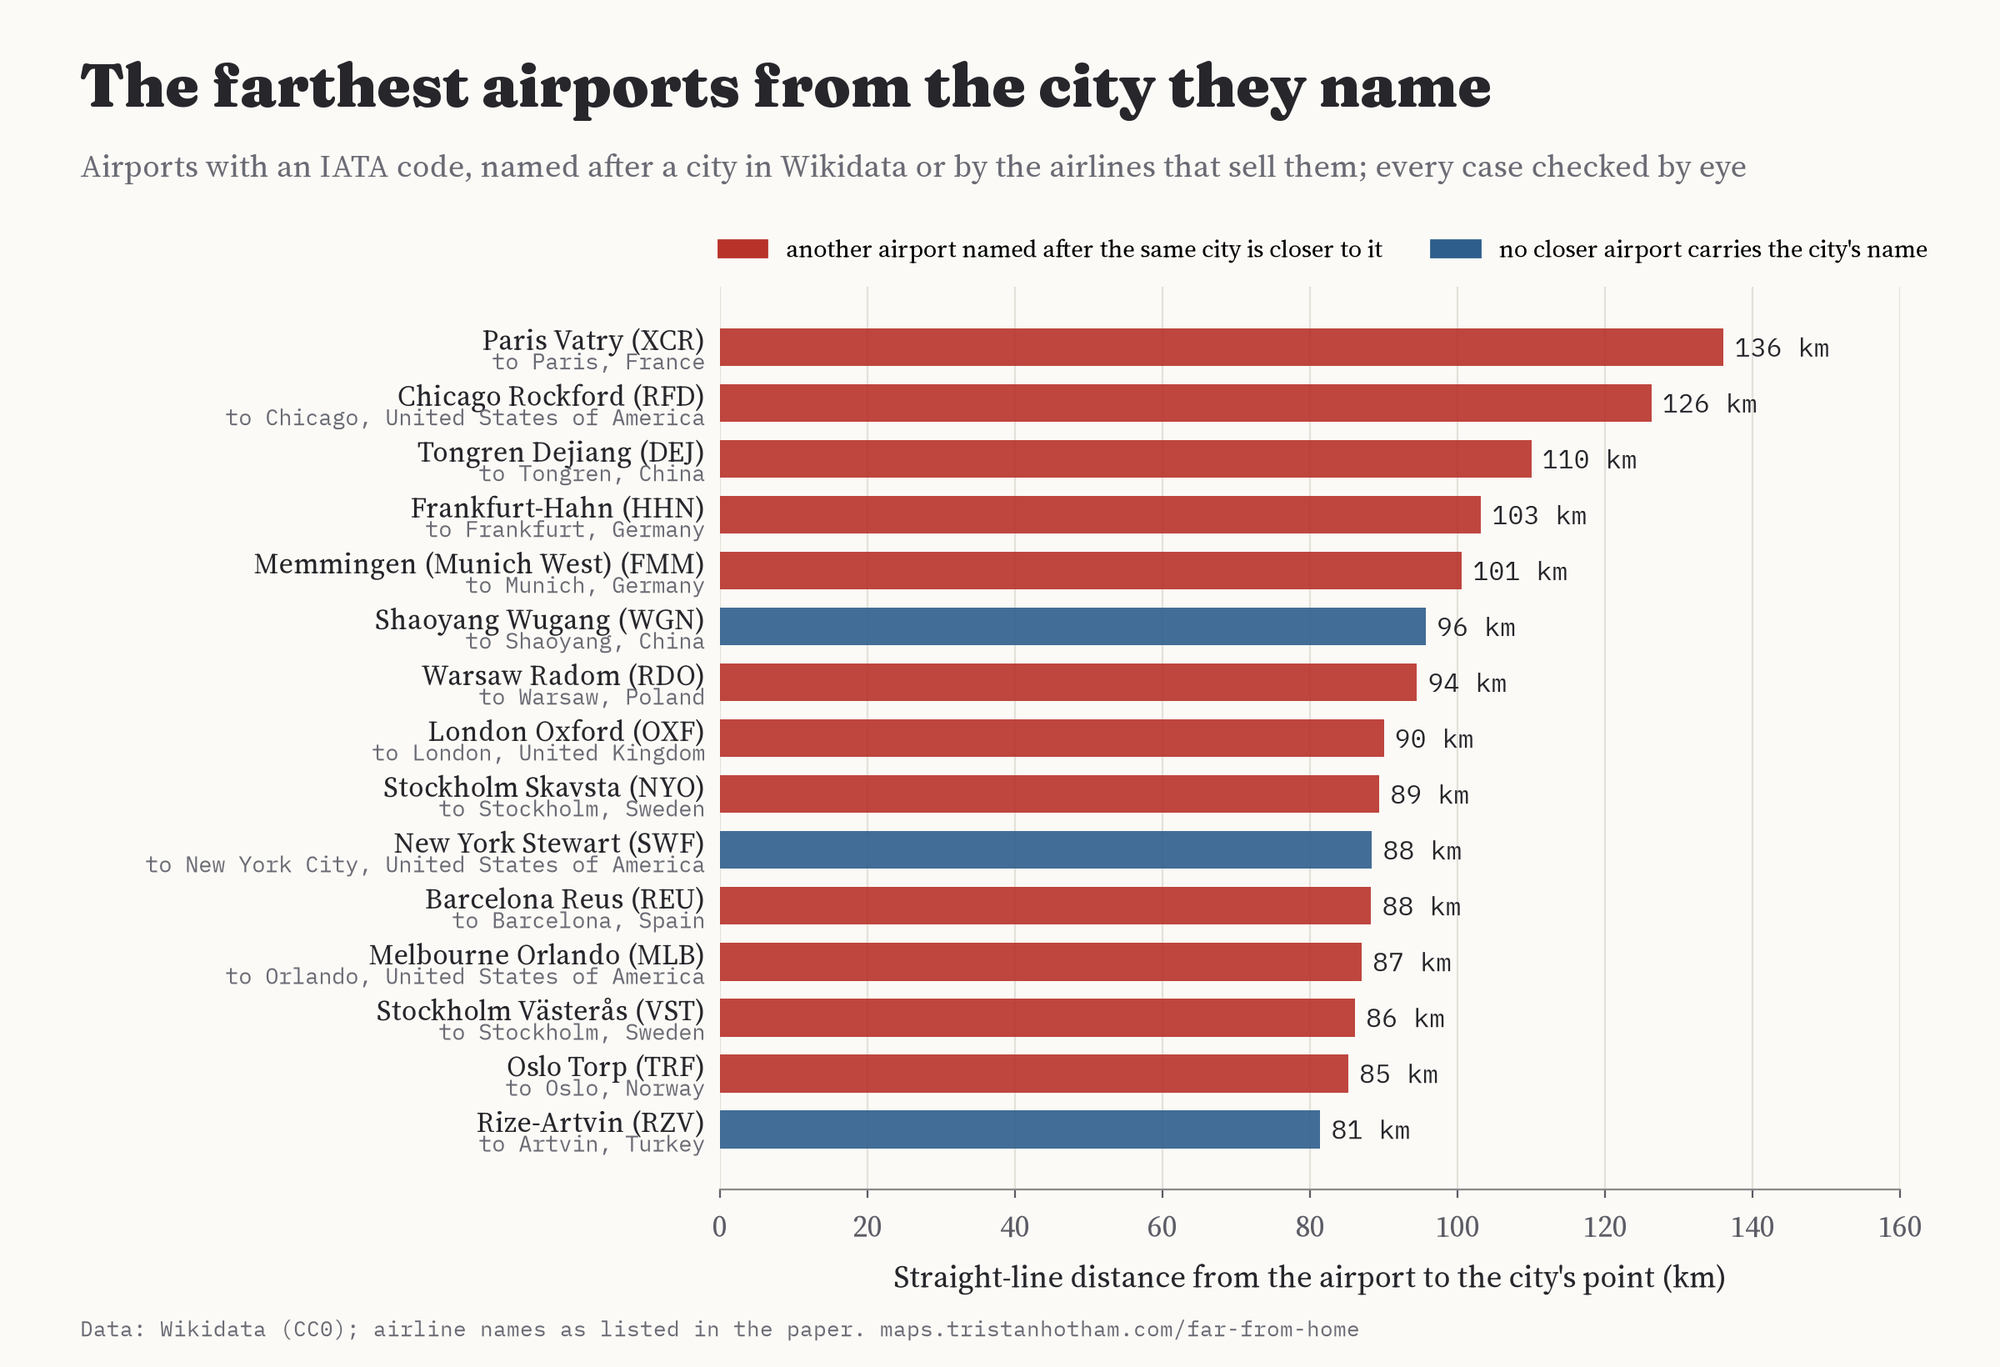
\includegraphics[width=\linewidth]{f_world.png}\caption{The fifteen airports farthest from the place they are named after.}\label{fig:world}\end{figure}

\begin{table}[tbp]\centering\small\caption{The fifteen airports farthest from the place they are named after (IATA code; kept cases). Second: another airport named after the same city is closer to it. Passengers: largest annual value in Wikidata.}\label{tab:world}\begin{tabular}{rp{6.2cm}p{2.8cm}rcr}\toprule & Airport (name sold by airlines in place of the label, where used) & Named after & km & Second & Passengers\\\midrule
1 & Paris Vatry (XCR) & Paris & 136.1 & yes & 132,972\\
2 & Chicago Rockford International Airport (RFD) & Chicago & 126.3 & yes & 224,432\\
3 & Tongren Dejiang Airport (DEJ) & Tongren & 110.0 & yes & \\
4 & Frankfurt-Hahn (HHN) & Frankfurt & 103.2 & yes & 1,860,000\\
5 & Memmingen (Munich West) (FMM) & Munich & 100.6 & yes & 3,200,000\\
6 & Shaoyang Wugang Airport (WGN) & Shaoyang & 95.7 &  & 59,571\\
7 & Warsaw Radom Airport (RDO) & Warsaw & 94.5 & yes & 9,903\\
8 & London Oxford Airport (OXF) & London & 90.0 & yes & 120\\
9 & Stockholm Skavsta Airport (NYO) & Stockholm & 89.4 & yes & 555,622\\
10 & New York Stewart International Airport (SWF) & New York City & 88.4 &  & 690,411\\
11 & Barcelona Reus (REU) & Barcelona & 88.3 & yes & 911,827\\
12 & Melbourne Orlando International Airport (MLB) & Orlando & 87.0 & yes & 465,082\\
13 & Stockholm Västerås Airport (VST) & Stockholm & 86.1 & yes & 93,080\\
14 & Oslo Torp (TRF) & Oslo & 85.2 & yes & 2,073,228\\
15 & Rize-Artvin Airport (RZV) & Artvin & 81.4 &  & 524,694\\
\bottomrule\end{tabular}\end{table}

Europe has more of the far cases than any other continent (15 of the 33 airports 50 km or more from their namesake; Figure~\ref{fig:europe}), almost all of them airports sold by low-cost airlines under a big city's name: Paris Beauvais (68.7 km), Barcelona Reus (88.3 km) and Girona (75.4 km), Düsseldorf Weeze (60.8 km), Hamburg Lübeck (55.2 km), Milan Bergamo (45.4 km) and Brussels South Charleroi (43.7 km). Relative to city size, the most stretched are smaller cities with a distant airport: Melbourne Orlando is 14.6 notional city radii from Orlando, Samaná El Catey 12.6 from Samaná, and Frankfurt-Hahn, fourth, 11.5 from Frankfurt.

\begin{figure}[tbp]\centering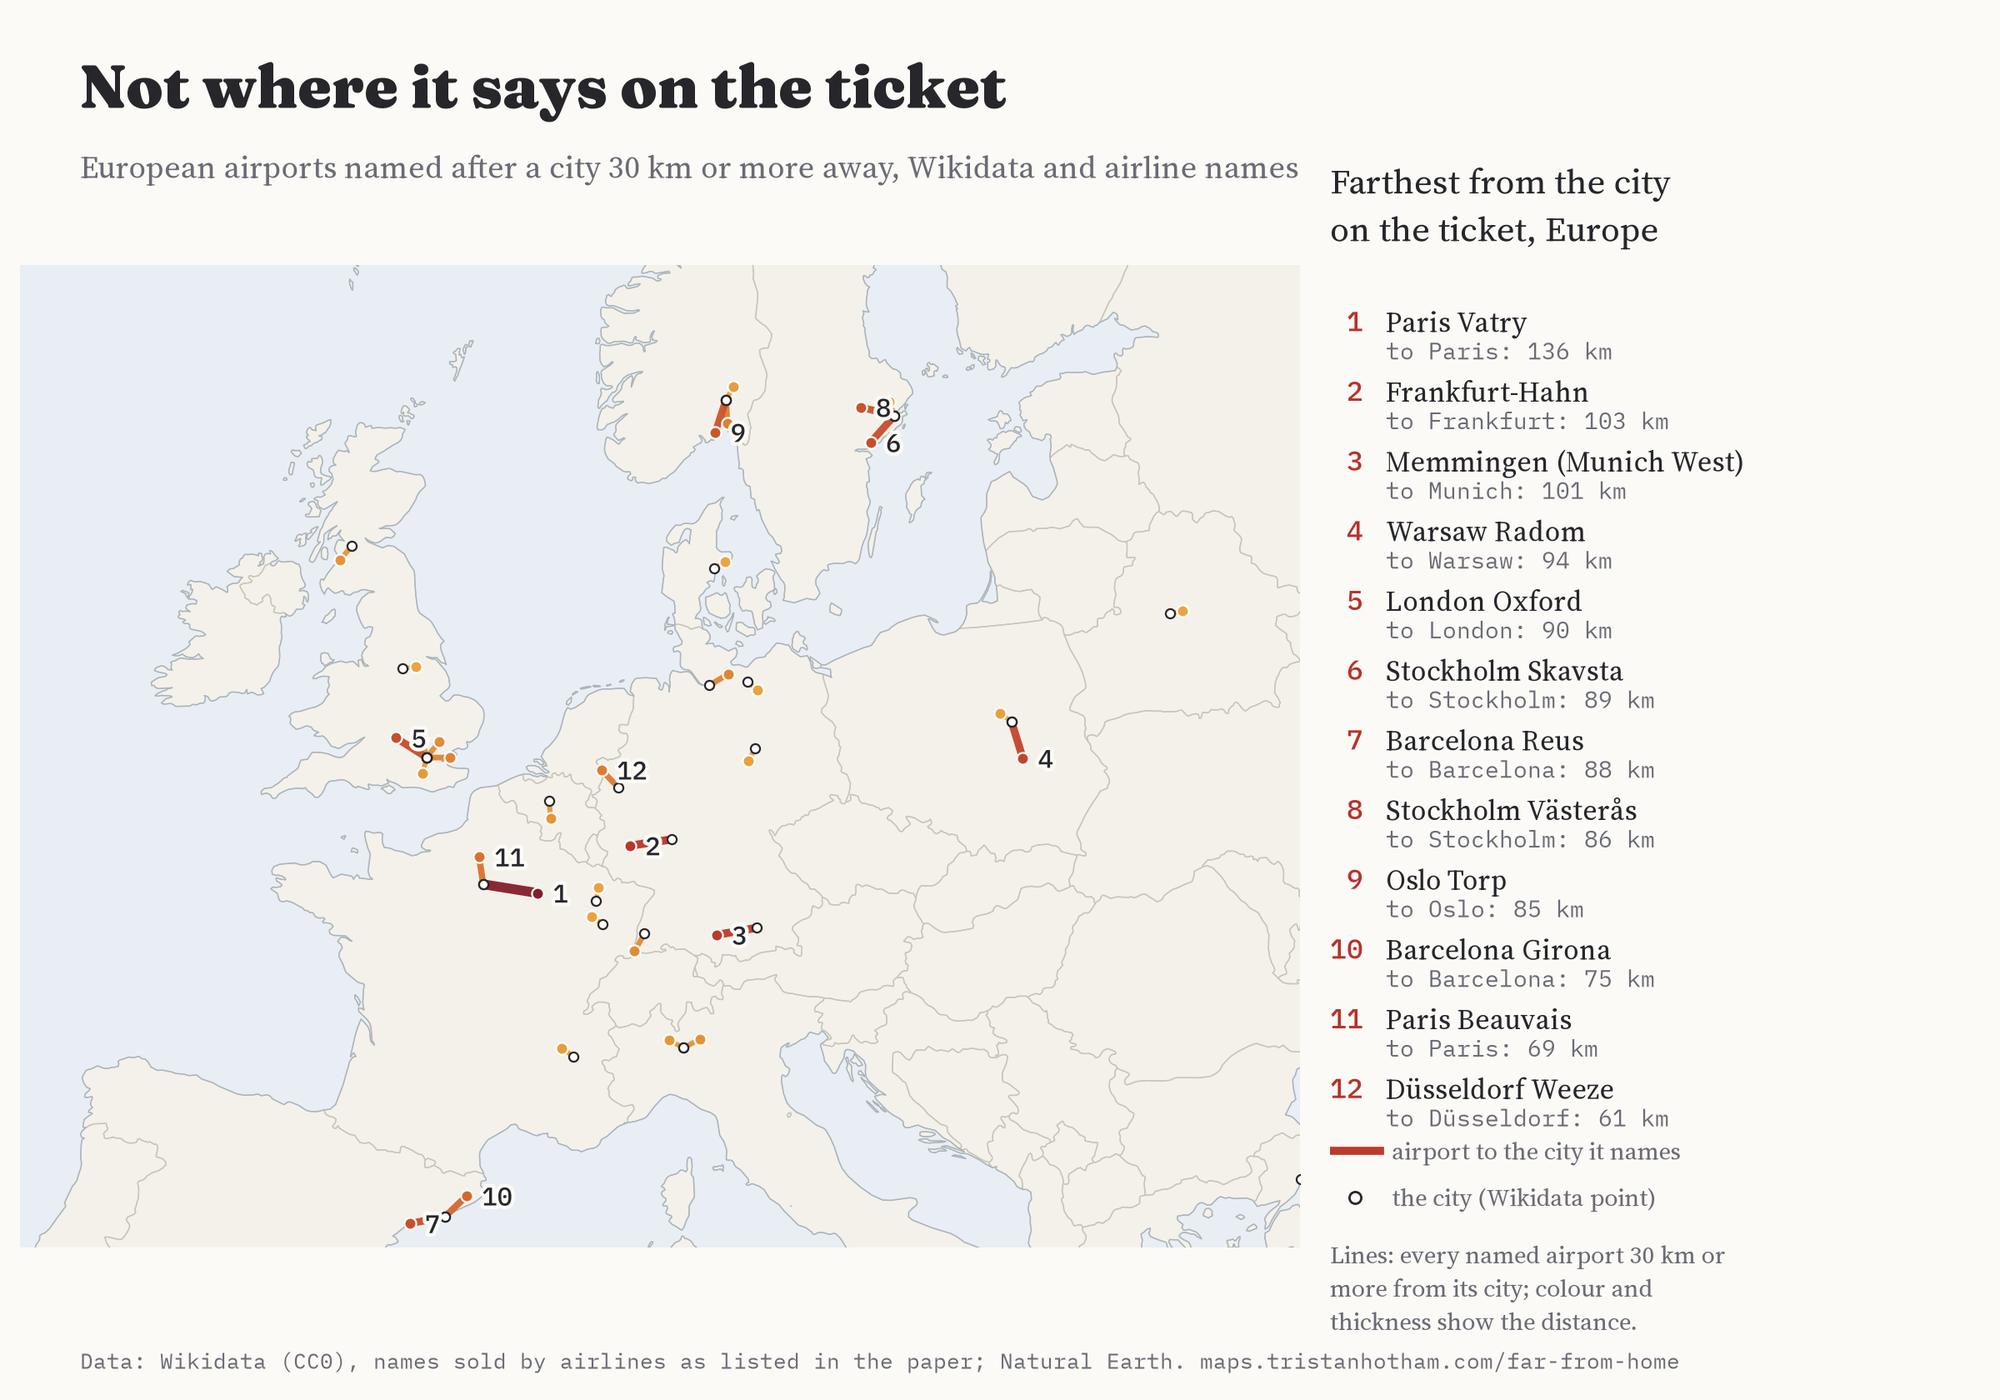
\includegraphics[width=\linewidth]{f_europe.png}\caption{European airports 30 km or more from the city they are named after.}\label{fig:europe}\end{figure}

\subsection{Britain and Ireland}
London stretches furthest: London Oxford Airport, at Kidlington, is 90.0 km from London, London Southend 57.2 km, Stansted 48.9 km, Luton 44.1 km, Gatwick 40.3 km and Heathrow 23.4 km. Outside London the farthest are Glasgow Prestwick (44.7 km from Glasgow) and Doncaster Sheffield (32.6 km from Sheffield). Airports in the Republic of Ireland all lie within 8 km of their towns; those with wider names are named after a county or region (Donegal, Connemara) and are excluded as regions, as are island airports such as the Isle of Man, Jersey, Guernsey and Islay.

\begin{table}[tbp]\centering\small\caption{Airports in Britain and Ireland farthest from the place they are named after.}\label{tab:uk}\begin{tabular}{rp{6.2cm}p{2.8cm}rcr}\toprule & Airport (name sold by airlines in place of the label, where used) & Named after & km & Second & Passengers\\\midrule
1 & London Oxford Airport (OXF) & London & 90.0 & yes & 120\\
2 & London Southend Airport (SEN) & London & 57.2 & yes & 2,035,535\\
3 & London Stansted Airport (STN) & London & 48.9 & yes & 23,319,523\\
4 & Glasgow Prestwick Airport (PIK) & Glasgow & 44.7 & yes & 444,433\\
5 & London Luton Airport (LTN) & London & 44.1 & yes & 13,322,236\\
6 & London Gatwick Airport (LGW) & London & 40.3 & yes & 40,899,000\\
7 & Doncaster Sheffield Airport (DSA) & Sheffield & 32.6 & yes & 959,321\\
8 & London Heathrow Airport (LHR) & London & 23.4 & yes & 83,884,572\\
9 & London Biggin Hill Airport (BQH) & London & 22.5 & yes & 4,002\\
10 & Belfast International Airport (BFS) & Belfast & 19.6 & yes & 4,818,214\\
\bottomrule\end{tabular}\end{table}

\subsection{Stations}
Of 3,576 stations, 2,888 (80.8\%) have a name that begins with a UK settlement in Wikidata. Half lie within 0.58 km of it; 169 (5.9\%) lie 2 km or more away and 15 lie 5 km or more (Figure~\ref{fig:stmap}). Measured from the settlement's centre, the farthest are airport stations: Manchester Airport (12.8 km), Birmingham International (12.4 km), London City Airport (12.2 km) and Inverness Airport (11.6 km). These airport stations are named after the airport, not the town, and inherit its distance, so they are left out of the ranking beyond the town. Measured beyond a notional circle round the settlement, Tiverton Parkway leads (7.6 km beyond, 9.1 km from Tiverton), then Llanbister Road (6.7 km), Dent (5.8 km) and Beaulieu Road (5.5 km) (Table~\ref{tab:st}).

\begin{figure}[tbp]\centering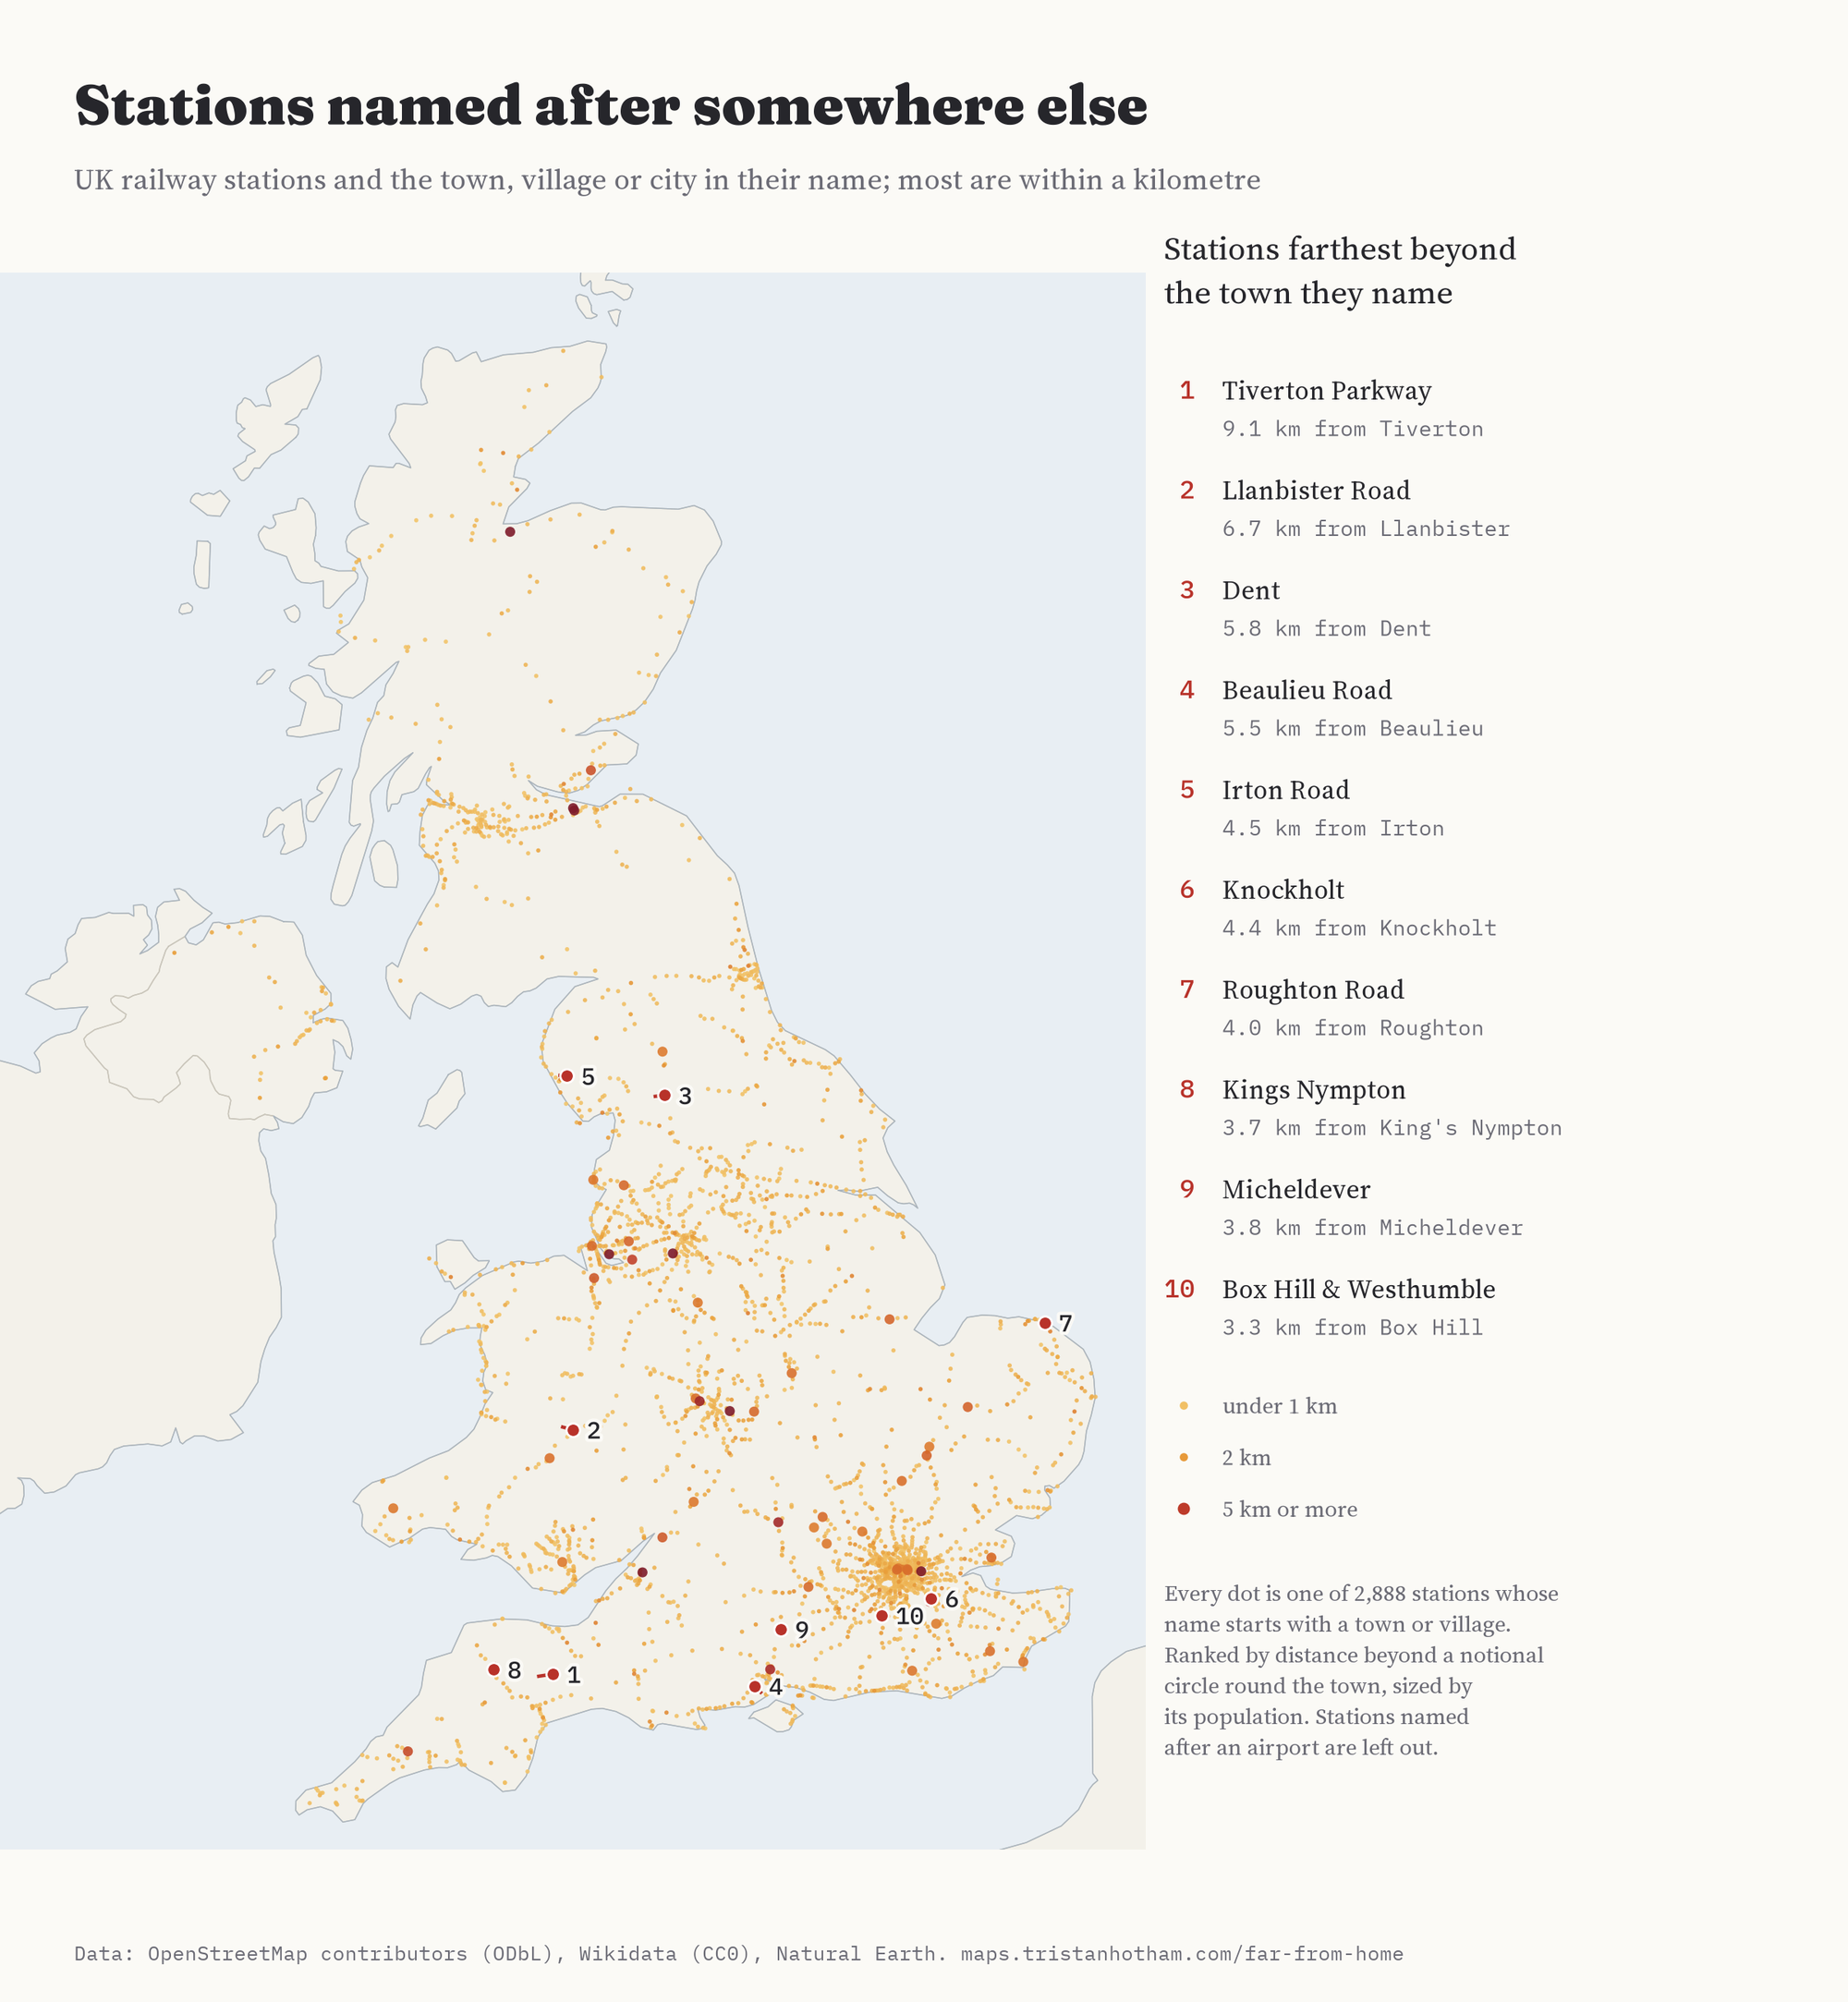
\includegraphics[width=0.92\linewidth]{f_stations_map.png}\caption{UK stations by distance to the settlement in their name; the ten farthest beyond a notional circle round the settlement, airport stations aside, are numbered.}\label{fig:stmap}\end{figure}

\begin{table}[tbp]\centering\small\caption{UK stations farthest beyond a notional circle round the settlement in their name (3,000 people per km$^2$). km: from the settlement's point.}\label{tab:st}\begin{tabular}{rllp{3.2cm}rr}\toprule & Station & CRS & Named after & km & Beyond circle\\\midrule
1 & Tiverton Parkway & TVP & Tiverton & 9.1 & 7.6\\
2 & Llanbister Road & LLT & Llanbister & 6.7 & 6.5\\
3 & Dent & DNT & Dent & 5.8 & 5.5\\
4 & Beaulieu Road & BEU & Beaulieu & 5.5 & 5.2\\
5 & Irton Road &  & Irton & 4.5 & 4.5\\
6 & Knockholt & KCK & Knockholt & 4.4 & 4.0\\
7 & Roughton Road & RNR & Roughton & 4.0 & 3.6\\
8 & Kings Nympton & KGN & King's Nympton & 3.7 & 3.5\\
9 & Micheldever & MIC & Micheldever & 3.8 & 3.4\\
10 & Box Hill \& Westhumble & BXW & Box Hill & 3.3 & 3.3\\
11 & Cam and Dursley & CDU & Dursley & 4.1 & 3.2\\
12 & Swineshead & SWE & Swineshead & 3.8 & 3.2\\
\bottomrule\end{tabular}\end{table}

There are 82 stations with ``Road'' in their name (62 with a CRS code). Many are named after streets, as in London (Tottenham Court Road, Wandsworth Road) and Manchester (Oxford Road), and 7 matches were rejected as streets in the checks. 9 are named after a village 2 km or more away (Figure~\ref{fig:kinds}): Llanbister Road, Beaulieu Road, Irton Road, Roughton Road, Wittersham Road, Builth Road, Clarbeston Road, Farningham Road and Harling Road. The 25 parkways have a median distance of 2.2 km; the farthest are Tiverton Parkway, Liverpool South Parkway (8.8 km) and Bristol Parkway (7.7 km).

\begin{figure}[tbp]\centering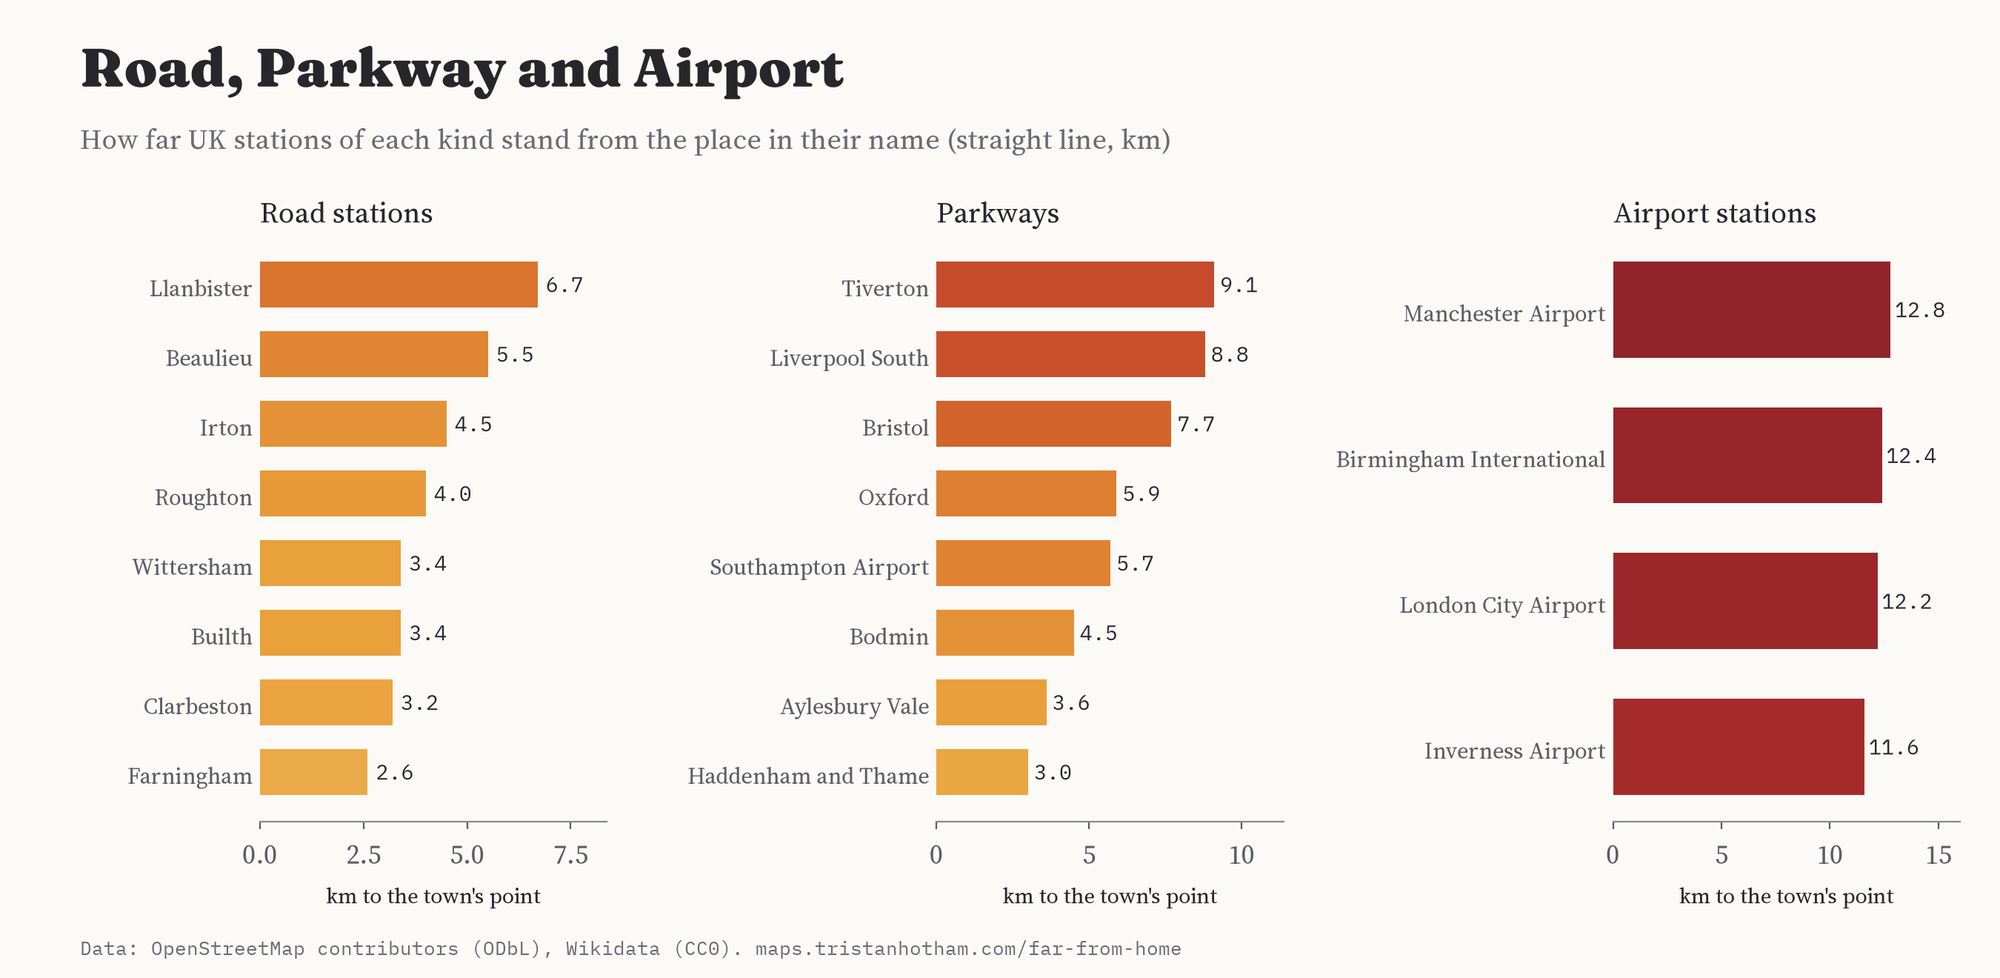
\includegraphics[width=\linewidth]{f_kinds.png}\caption{Distance to the settlement in the name for Road stations, parkways and airport stations.}\label{fig:kinds}\end{figure}

\subsection{What the checks found}
Of the 113 airport cases of 40 km or more, 66 were kept, 23 (20.4\%) were wrong links or coordinates, 12 named a region, island, county or country, and 12 could not be settled and were left out (Figure~\ref{fig:checks}). The wrong links are mostly to another place of the same name: Bathurst Island Airfield in the Northern Territory linked to Bathurst in New South Wales, Wilmington International in North Carolina linked to Wilmington in Delaware, Ibaraki Airport linked to Ibaraki city in Osaka rather than the prefecture, and pairs of Yichuns, Qianjiangs, Zhijiangs, Nagoyas and Heringsdorfs. Of the 286 station matches of 3 km or more, 60 were kept, 208 were a different place of the same name or a station named after a district, valley or estate, 7 were streets, 7 were coordinate errors and 4 were unsure. All 183 station matches of 40 km or more were coincidences, usually because the station's real namesake is missing from the settlement list under that name.

\begin{figure}[tbp]\centering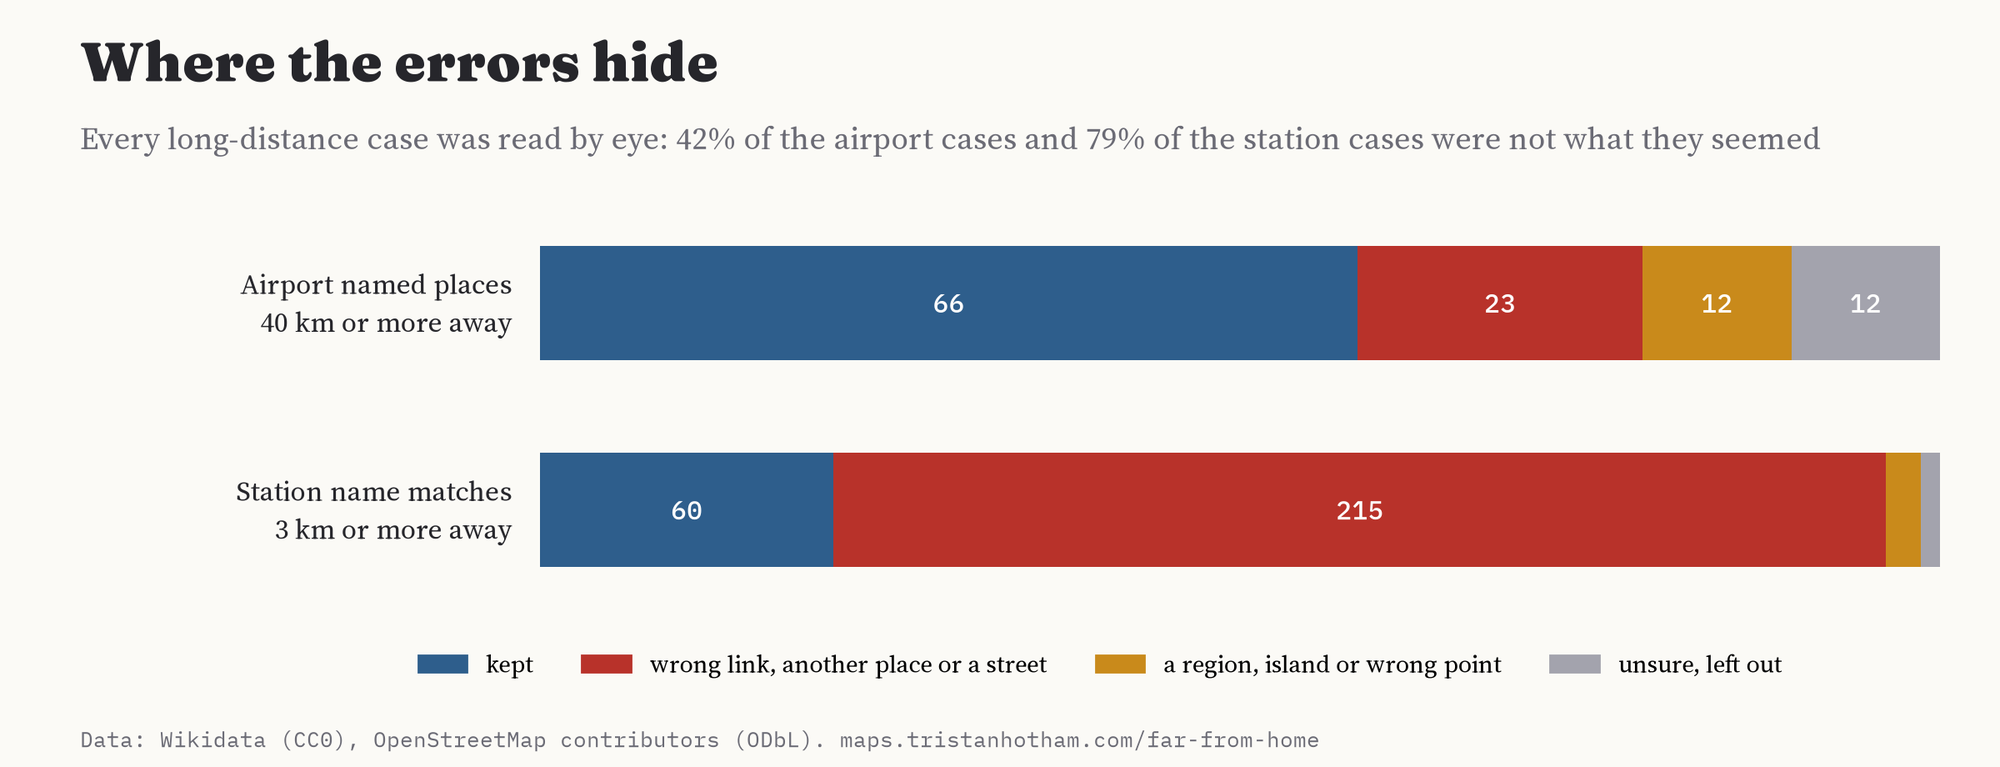
\includegraphics[width=\linewidth]{f_checks.png}\caption{Verdicts from reading every long case by eye.}\label{fig:checks}\end{figure}

\section{Limitations}
Straight-line distance from a point to a point is a crude measure: it ignores roads and rail, and a city's point in Wikidata is its centre, not its edge. Populations are those of the administrative unit (the city of Paris, not its region) and the notional circles assume a uniform density. Wikidata's places served and its UK settlement list are incomplete: an airport whose namesake is not linked, or whose name differs from the label of the place, is not measured, and some stations go unmatched (Bradford in West Yorkshire is missing from the settlement list). The marketing names are a short list from my own knowledge of how these airports were sold, each checked against airline or airport listings; others exist, names change, and several of these airports have since dropped the big city's name. Cases under 40 km (airports) and 3 km (stations) were not read by eye. Wikidata keeps closed airports (Oslo Fornebu, closed in 1998; Doncaster Sheffield, closed in 2022), and they count when deciding whether a city has a closer airport. Some verdicts rest on judgement, especially the regions and the unsure cases.

\section{Conclusion}
Most airports and stations are close to the place in their name: a few kilometres for airports, a few hundred metres for stations. The far cases are few and of a few kinds: second airports sold under a big city's name, often former military fields; Chinese airports named after their prefecture; airport stations and parkways; and the Victorian Road stations. Finding them in open data requires reading every long case, because at the head of a distance ranking most of what the data first says is wrong.

\section*{Data and code availability}
The interactive map is at \url{https://maps.tristanhotham.com/far-from-home/}. Code, the overrides and the derived tables are at \url{https://github.com/Tristan-Hotham/far-from-home} and archived with this paper at https://doi.org/10.5281/zenodo.24087597. Airport data are from Wikidata (CC0); station data are derived from OpenStreetMap (\copyright{} OpenStreetMap contributors) and released under the Open Database Licence; Natural Earth is public domain; text and figures CC BY 4.0; code MIT.

\section*{AI statement}
I wrote the text, with drafting and editing assistance from Claude (Anthropic), which also helped prepare the analysis code. I reviewed and checked all text and results.

\begin{thebibliography}{10}
\bibitem[Bast and Buchhold(2017)]{bast2017} Bast, H. and Buchhold, B. (2017) QLever: a query engine for efficient SPARQL+Text search. \textit{Proceedings of the 2017 ACM Conference on Information and Knowledge Management (CIKM)}, 647 to 656.
\bibitem[Haklay and Weber(2008)]{haklay2008} Haklay, M. and Weber, P. (2008) OpenStreetMap: user-generated street maps. \textit{IEEE Pervasive Computing} 7(4), 12 to 18.
\bibitem[Natural Earth(2026)]{naturalearth} Natural Earth (2026) Free vector and raster map data at 1:10m, 1:50m and 1:110m scales. \url{https://www.naturalearthdata.com/}.
\bibitem[Vrandečić and Krötzsch(2014)]{vrandecic2014} Vrandečić, D. and Krötzsch, M. (2014) Wikidata: a free collaborative knowledgebase. \textit{Communications of the ACM} 57(10), 78 to 85.
\end{thebibliography}

\appendix
\section{Names sold by airlines}
\begin{small}\begin{longtable}{lp{3.2cm}lrp{6.4cm}}\caption{Names under which airlines have sold secondary airports, used as namesakes in addition to the data (from the author's knowledge, each checked against airline or airport listings). km: distance in the data.}\label{tab:mk}\\\toprule IATA & Sold as & City & km & Note\\\midrule\endhead
HHN & Frankfurt-Hahn & Frankfurt & 103.2 & The airport's own name for most of its life, and the name airlines sold it under; Wikidata now labels it Hahn Airport\\
BVA & Paris Beauvais & Paris & 68.7 & Sold by airlines as Paris Beauvais; Wikidata label Beauvais-Tillé Airport\\
XCR & Paris Vatry & Paris & 136.1 & Marketed as Paris-Vatry; Wikidata label Châlons Vatry Airport\\
REU & Barcelona Reus & Barcelona & 88.3 & Sold by airlines as Barcelona (Reus); Wikidata label Reus Airport\\
GRO & Barcelona Girona & Barcelona & 75.4 & Sold by airlines as Barcelona (Girona); Wikidata label Girona-Costa Brava Airport\\
FMM & Memmingen (Munich West) & Munich & 100.6 & Sold by airlines as Memmingen (Munich West); Wikidata label Memmingen Airport\\
NRN & Düsseldorf Weeze & Düsseldorf & 60.8 & The airport's own name until it reverted to Weeze; Wikidata label Niederrhein Airport\\
TRF & Oslo Torp & Oslo & 85.2 & Sold by airlines as Oslo Torp (Sandefjord); Wikidata label Sandefjord Airport\\
LBC & Hamburg Lübeck & Hamburg & 55.2 & Sold by airlines as Hamburg Lübeck; Wikidata label Lübeck-Blankensee Airport\\
TSF & Venice Treviso & Venice & 25.7 & Sold by airlines as Venice Treviso; Wikidata label Treviso Airport\\
BGY & Milan Bergamo & Milan & 45.4 & Sold by airlines as Milan Bergamo; Wikidata label Bergamo-Il Caravaggio\\
\bottomrule\end{longtable}\end{small}
\end{document}
